
\section{DSS To DWH}

\begin{breakbox}
\boxtitle{Grouping Sets:}
\sql{sql_code/grouping_sets.sql}
Bemerkungen:
\begin{itemize}
	\item PARTITION BY $\cdots$: Wenn weggelassen, werden alle Tupel selected.
	\item ORDER BY $\cdots$: Sortiert die Sequenz.
	\item $\cdots$ ROWS $\cdots$: (optional): Wenn window size nicht explizit gegeben:
		\begin{itemize}
			\item ganze Partition oder
			\item bis zu diesem Tupel für den Fall, dass eine Sortiersequenz gegeben ist.
		\end{itemize}
\end{itemize}
\end{breakbox}

\begin{breakbox}
\boxtitle{SUM über Partitionen:}
\sql{sql_code/multiple_sums.sql}
\end{breakbox}

\begin{breakbox}
\boxtitle{LAG:}
\sql{sql_code/lag.sql}
\end{breakbox}

\begin{breakbox}
\boxtitle{RANK:}
\sql{sql_code/rank.sql}
\end{breakbox}

\begin{breakbox}
\boxtitle{AVG und Formatierung:}
\sql{sql_code/avg_format.sql}
\end{breakbox}

%\begin{breakbox}
%\boxtitle{Analytische Aggregatoren:}
%\begin{center}
%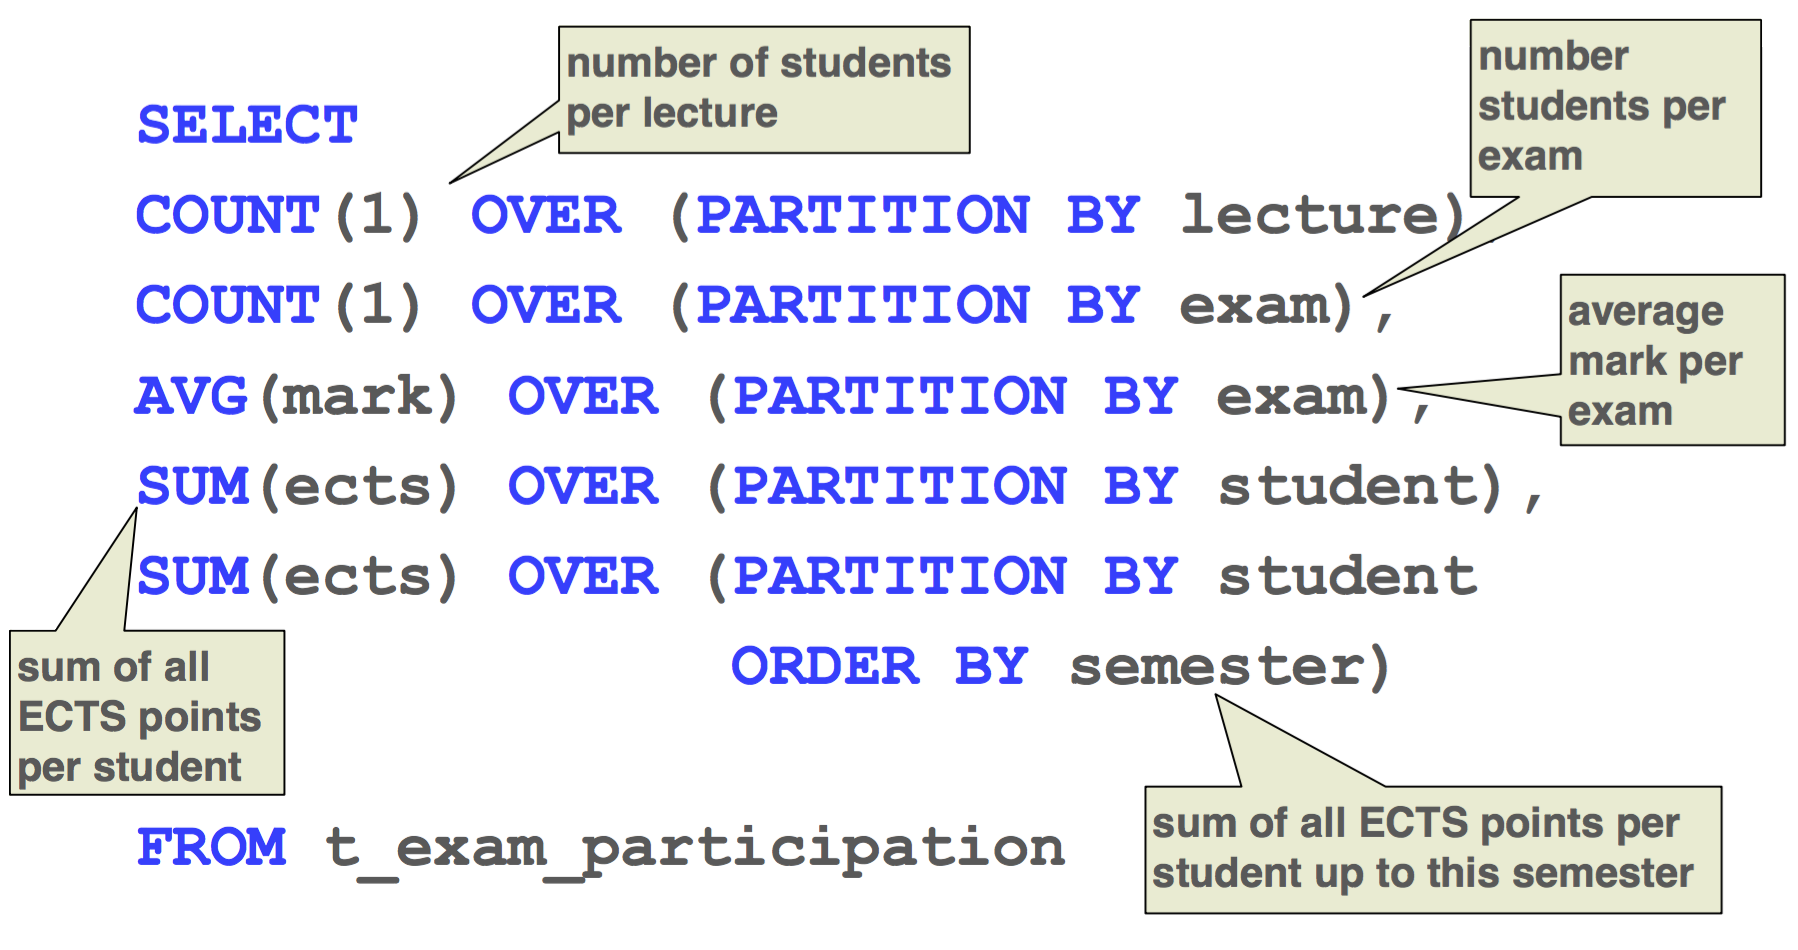
\includegraphics[width=.12\textwidth]{slides_images/analytical_aggregate_functions.png}
%\end{center}
%\end{breakbox}

\begin{breakbox}
\boxtitle{Zusätzliche analytische Funktionen:}
\begin{itemize}
	\item VAR\_POP(), VAR\_SAMP(), STDDEV\_POP(), STDDEV\_SAMP()
	\begin{itemize}
		\item determine variance and standard dviation
	\end{itemize}
	\item RANK(), DENSERANK()
	\begin{itemize}
		\item establish a ranking - with or w/o gaps
	\end{itemize}
	\item FIRST\_VALUE(), LAST\_VALUE()
	\begin{itemize}
		\item gives first (last) value of a sort sequence
	\end{itemize}
	\item CORR()
	\begin{itemize}
		\item calculate correlation
	\end{itemize}
	\item LAG(), LEAD()
	\begin{itemize}
		\item go back (lag) / advance (lead) n records in partition
	\end{itemize}
	\item RATIO\_TO\_REPORT()
	\begin{itemize}
		\item value's proportion of total of partition
	\end{itemize}
	\item NTILE()
	\begin{itemize}
		\item divides each partition in n like fractions (quarters, tenths, halves etc.)
	\end{itemize}
\end{itemize}	
\end{breakbox}

\begin{breakbox}
\boxtitle{OLTP vs. OLAP:}
\begin{itemize}
	\item Workload:
	\begin{itemize}
		\item OLTP: predictable / constantly high
		\item OLAP: unpredictable / erratic
	\end{itemize}
	\item Units of work / Transactions:
	\begin{itemize}
		\item OLTP: small / often writing
		\item OLAP: large, only reading
	\end{itemize}
	\item Performance / Requirements:
	\begin{itemize}
		\item OLTP: strict
		\item OLAP: varying
	\end{itemize}
	\item Queries:
	\begin{itemize}
		\item OLTP: simply structured
		\item OLAP: complex
	\end{itemize}
\end{itemize}
\end{breakbox}
